\documentclass{article}

% Language setting
% Replace `english' with e.g. `spanish' to change the document language
\usepackage[english]{babel}

% Set page size and margins
% Replace `letterpaper' with `a4paper' for UK/EU standard size
\usepackage[letterpaper,top=2cm,bottom=2cm,left=3cm,right=3cm,marginparwidth=1.75cm]{geometry}

% Useful packages
\usepackage{enumerate}
\usepackage[shortlabels]{enumitem}
\usepackage{amsmath, amsfonts, amssymb, mathtools}
\usepackage{graphicx}
\usepackage[colorlinks=true, allcolors=blue]{hyperref}
\usepackage[table]{xcolor}  % For coloring rows
\usepackage{ tipa }
\usepackage[section]{placeins}
\usepackage{float} % For 'H' option of images

% For drawing state machine
\usepackage{tikz}
\usetikzlibrary{automata} % Import library for drawing automata
\usetikzlibrary{positioning} % ...positioning nodes
\usetikzlibrary{arrows} % ...customizing arrows
\tikzset{
    node distance=3cm, % Minimum distance between two nodes. Change if necessary.
    every state/.style={ % Sets the properties for each state
        thick,
        fill=gray!10
    },
    initial text={}, % No label on start arrow
    double distance=2pt, % Adjust appearance of accept states
    bend angle=15,
    every edge/.style={ % Sets the properties for each transition
        draw,
        ->,>=stealth, % Makes edges directed with bold arrowheads
        auto,
        thick
    }
}
            
\let\epsilon\varepsilon

\newcommand{\N}{\mathbb{N}}

\title{
Cyber Physical Systems - Discrete Models \\
[0.2em]Exercise Sheet 7 Solution
}
\author{
  Alper Ari\\
  \texttt{aa508@uni-freiburg.edu}
  \and
  Onur Sahin\\
  \texttt{os141@uni-freiburg.de}
}
\date{\today}

\begin{document}
\maketitle

\section*{Exercise 1:  Linear-Time Properties}
\begin{enumerate}
    \item Property $P_1:$
    \begin{enumerate}[i]
        \item 
        $
            \{ A_0 A_1 A_2 ... | \forall i \in \N \cdot a\in A_i \vee b\in A_i \}
        $
        \item 
        $
            \{a\}(\{a\}\{a,b\})^\omega
        $
        \item 
        $
            \{a\} \emptyset (\{a\}\{a,b\})^\omega
        $
        \item 
        $
            T \nvDash P_1 \text{ because not all of the traces satisfy $P_1$ (example above)}.
        $
    \end{enumerate}

    \item Property $P_2:$
    \begin{enumerate}[i]
        \item 
        $
            \{ A_0 A_1 A_2 ... | \forall i \in \N \cdot a\in A_i \wedge b\in A_i \}
        $
        \item 
        $
            -
        $
        \item 
        $
            \{a\} \emptyset (\{a\}\{a,b\})^\omega
        $
        \item 
        $
            T \nvDash P_2 \text{ because none of the traces satisfy $P_2$ (example above)}.
        $
    \end{enumerate}

    \item Property $P_3:$
    \begin{enumerate}[i]
        \item 
        $
            \{ A_0 A_1 A_2 ... | \forall i \in \N \cdot (b\in A_i \longrightarrow \exists j \in \N \cdot j \leq i \cdot a \in A_j) \}
        $
        \item 
        $
            \{a\} (\{a\}\{a,b\})^\omega
        $
        \item 
        $
            -
        $
        \item 
        $
            T \vDash P_3 \text{ because all traces satisfy $P_3$}.
        $
    \end{enumerate}

    \item Property $P_4:$
    \begin{enumerate}[i]
        \item 
        $
            \{ A_0 A_1 A_2 ... | \forall i \in \N \cdot (a \in A_i \longrightarrow \exists j \in \N \cdot j \geq i \cdot b\in A_j) \}
        $
        \item 
        $
            \{a\} (\{a\}\{a,b\})^\omega
        $
        \item 
        $
            -
        $
        \item 
        $
            T \vDash P_4 \text{ because all traces satisfy $P_4$}.
        $
    \end{enumerate}

    \item Property $P_5:$
    \begin{enumerate}[i]
        \item 
        $
            \{ A_0 A_1 A_2 ... |\exists i,j,k \in \N \cdot (a\in A_i \wedge a\in A_j \wedge a\in A_k) \wedge (\forall z \in \N / \{i,j,k\}) \wedge (i \neq j \neq k) \cdot a\notin A_z \}
        $
        \item 
        $
            -
        $
        \item 
        $
            \{a\} \emptyset (\{a\}\{a,b\})^\omega
        $
        \item 
        $
            T \nvDash P_5 \text{ because no traces satisfy $P_5$}.
        $
    \end{enumerate}

    \item Property $P_6:$
    \begin{enumerate}[i]
        \item 
        $
            \{ A_0 A_1 A_2 ... |{\exists}^\infty i\in \N \cdot a\in A_i \Longrightarrow {\exists}^\infty j\in \N \cdot b\in A_j \}
        $
        \item 
        $
            \{a\} (\{a\}\{a,b\})^\omega
        $
        \item 
        $
            -
        $
        \item 
        $
            T \vDash P_6 \text{ because all traces satisfy $P_6$}.
        $
    \end{enumerate}

    \item Property $P_7:$
    \begin{enumerate}[i]
        \item 
        $
            \{ A_0 A_1 A_2 ... |\exists i \in \N \cdot \forall j\in \N \cdot j\geq i \cdot a\notin A_j \}
        $
        \item 
        $
            -
        $
        \item 
        $
            \{a\} \emptyset (\{a\}\{a,b\})^\omega
        $
        \item 
        $
            T \nvDash P_7 \text{ because no traces satisfy $P_7$}.
        $
    \end{enumerate}
\end{enumerate}


\newpage
\section*{Exercise 2: Complement of LT-Properties}

\begin{enumerate}[(a)]
    \item \textbf{If $\tau \vDash \neg E$ holds, it follows that $\tau \nvDash E$ holds:}\\
    True. Proof by contradiction. Assume $\tau \vDash \neg E \wedge \tau \vDash E$. \\
    Then it follows that $\tau \in \neg E \wedge \tau \in E$. \\
    Since the fact that $E \cap \neg E = \emptyset$, the assumption contradicts.\\
    Therefore, if $\tau \vDash \neg E$ holds, it follows that $\tau \nvDash E$ holds.
    
    \item \textbf{If $\tau \nvDash \neg E$ holds, it follows that $\tau \vDash E$ holds:} \\
    True. Proof by contradiction. Assume $\tau \nvDash E \wedge \tau \nvDash \neg E$. \\
    Then $\tau \notin E \wedge \tau \notin \neg E$.\\
    This leads to $\tau \notin (E \cup \neg E)$ which actually means $\tau \notin (2^{AP})^\omega$ which is a contradiction.\\
    Therefore, if $\tau \nvDash \neg E$ holds, it follows that $\tau \vDash E$ holds.
    
    \item \textbf{If $T \vDash \neg E$ holds, it follows that $T \nvDash E$ holds:}\\
    False. A counter example would be $T = \emptyset$ which is a transition system without any traces.\\
    In this case the system has no trace which violates both $E$ and $\neg E$.\\
    So, the given statement is false.
    
    \item \textbf{If $T \nvDash \neg E$ holds, it follows that $T \vDash E$ holds:}\\
    False. A counter example would be $T$ with traces $\{ {a}^\omega , {b}^\omega \}$ and property E = "always b".\\
    Here, $T \nvDash \neg E$ is false because one of the traces already satisfies E.\\
    And, $T \vDash E$ is also false because one of the traces already doesn't satisfy E. \\
    So, the given statement is false.

\end{enumerate}

\newpage
\section*{Exercise 3: Invariant checking I}
\begin{figure}[H]
    \centering
    \includegraphics[width=5in]{images/03.png}
    \label{fig:03}
\end{figure}


\newpage
\section*{Exercise 4: Invariant checking II}
\begin{figure}[ht] % ’ht’ tells LaTeX to place the figure ’here’ or at the top of the page
        \centering % centers the figure
        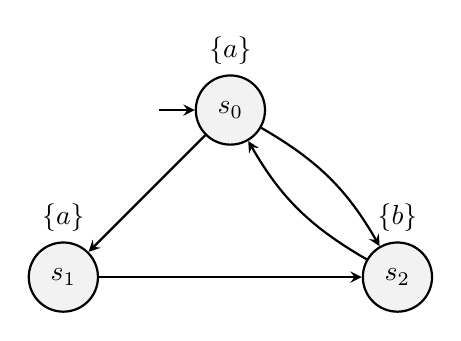
\begin{tikzpicture}
            \node[circle split, state, initial] (s0) [label=$\{a\}$] {$s_0$};
            \node[state, below left of=s0] (s1) [label=$\{a\}$] {$s_1$};
            \node[state, below right of=s0] (s2) [label=$\{b\}$] {$s_2$};
            
            \draw (s0) edge node {} (s1);
            \draw (s0) edge[bend left] node {} (s2);
            \draw (s2) edge[bend left] node {} (s0);
            \draw (s1) edge node {} (s2);

        \end{tikzpicture}
        \caption{Transition system with 3 states}
        \label{fig:state-machine-l1}
    \end{figure}
    
    $$\phi = a$$
    $$ \text{non-minimal} = \{s_0, s_1, s_2\}$$
    $$ \text{minimal} = \{s_0, s_2\}$$
    
\end{document}
